%\begin{figure*}[!t]
%        \centering
%	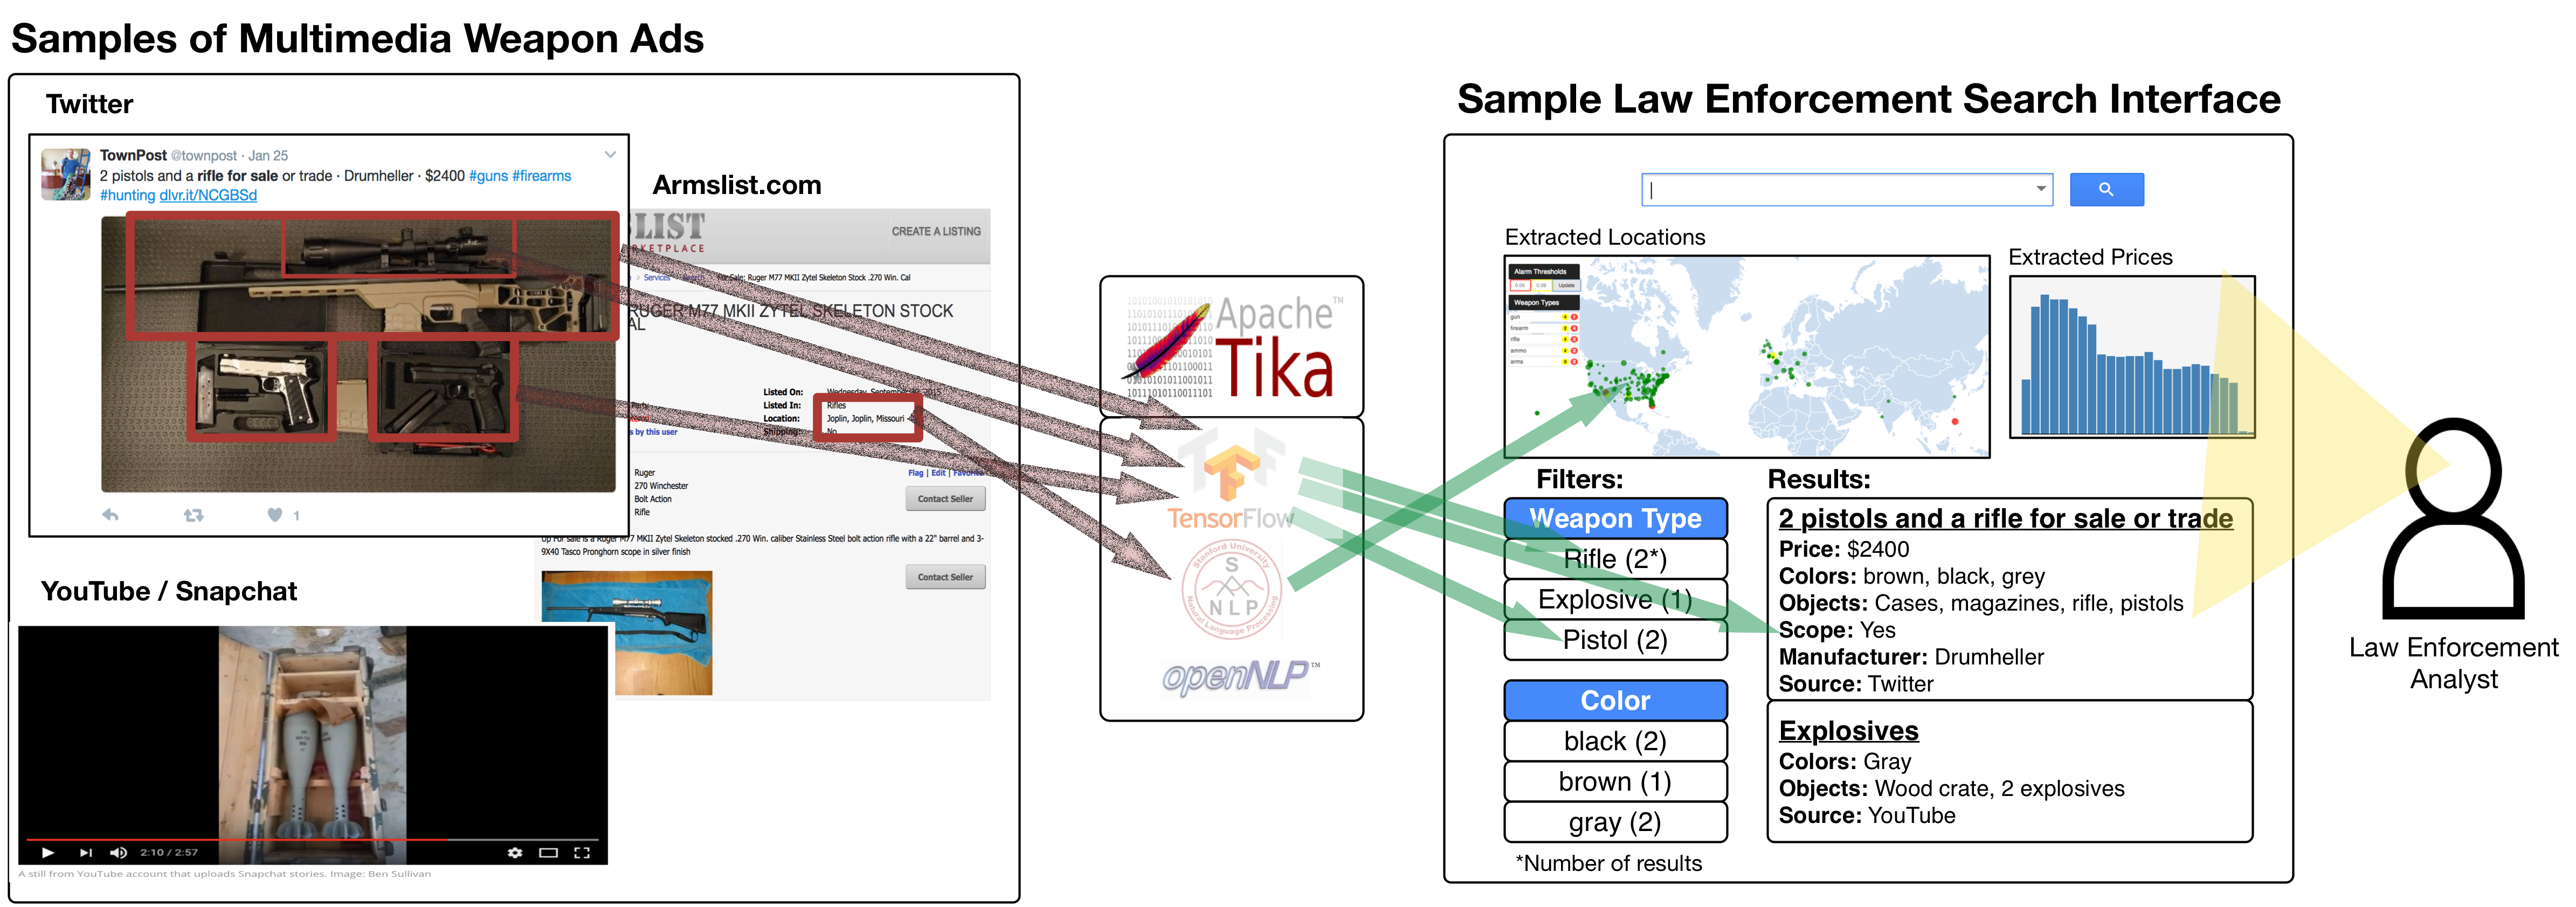
\includegraphics[width=\textwidth,height=6cm]{interface-diagram}
%	\caption{This diagram demonstrates how the integration of Tika and Tensorflow facilitates in-depth search across heterogenuous content types. There are several extensions to our object recognition implementation as well, including more refined categories, optical-character recognition, and image similarity metrics.}
%	\label{fig:interface-diagram}
%\end{figure*}
\section{Data Collection and Content Analysis in Memex}
\label{sec:memex-data}
% This section discusses motivations behind DARPA Memex and provides background on program data. 
Current commercial search engines provide generalized search interfaces that allow users to search across a limited portion of the web~\cite{fbo-memex}. However, in the context of cyber security and law enforcement, commercial search engines miss essential content from the Deep and Dark web. Because it is hard to reach, this content often harbors illicit activity. The goal of Memex is to develop software that can quickly and thoroughly collect, organize, and search subsets of information relevant to individual domains of interest. 

The program's initial focus was on human trafficking and the trade and sale of illicit goods, and several enhanced web crawlers were used to discover and retrieve information from the websites related to these domains. Along with the general-purpose web crawlers, specialized crawlers were used for the retrieval of Dark web data using The Onion Router (TOR) protocol \cite{mentor2016onion} and also specialized in the retrieval of dynamic AJAX content guarded by login forms. Fetched data were then cached within the system for analysis due to the ephemeral nature of the source (web) content.

% \subsection{Memex Dataset} \label{sec:memex-dataset}
The Memex data inlcuded 7.2 million items of content in the illegal weapon sales domain, of which 1.4 million objects were images. Before processing images, we analyzed the textual documents in a separate experiment using named-entity recognition (NER) models that extracted people, locations, organizations, weapon names, and weapon types. Tika has recently added support for this task using popular Natural Language Processing toolkits like Stanford CoreNLP\cite{Finkel:2005:INI:1219840.1219885}, Apache OpenNLP\cite{ApacheOpenNLP}, and MIT Lincoln Lab's MITIE \cite{MITIE-github}. However, as we described in Section 1, our work has focused on weapons images for two primary reaons: (1) web crawlers generally extract any linked content from a site and ensuring that images contain relevant objects was an important preprocessing step; and (2) classifying image objects allows for the cataloguing of specific objects of interest. 
With regard to number two, the queries we sought to answer were related to automated identification of (semi-)automatic weapons and illegal gun transactions -- this often requires direct analysis of the image rather than associated ad text. 

The ultimate goal of integrating and characterizing diverse content scattered across the web is to provide law enforcement analysts with tools that will help them quickly identify potentially illegal activity, and images and videos often provide salient information not available in text; in many cases, illegal weapons dealers intentionally embed revealing details in rich content mediums because they are harder to identify. This thinking coincides with the rise of weapons trafficking on social media platforms such as Snapchat, YouTube, and Instagram, where communication is centered around images and video \cite{socialmedia}. The integration of Tensorflow and Tika provides a single, streamlined platform that unites the extraction of textual and rich content. This combined content can then be exposed through search and visualization interfaces that improve analysts' abilities to drill-down and explore comprehensive, diverse content contained in weapons ads (see Figure \ref{fig:interface-diagram}). 

\begin{figure*}[!t]
        \includegraphics[width=\textwidth,height=5cm]{tensorflow-tika-integration}
        \caption{Tika and Tensorflow Integration}
        \label{fig:tf-tika-integration}
\end{figure*}

